\documentclass[11pt]{article}
\usepackage[utf8]{inputenc}
\usepackage[T1]{fontenc}
\usepackage{mathpazo}
\usepackage{microtype}
\usepackage[margin=1in]{geometry}
\usepackage{setspace}
\onehalfspacing
\usepackage{amsmath,amssymb}
\usepackage{graphicx}
\graphicspath{{figures/}}
\usepackage{booktabs}
\usepackage[round]{natbib}
\usepackage[colorlinks,citecolor=black,linkcolor=black,urlcolor=blue]{hyperref}

\title{\textbf{Phase-Locking Without Prediction}\\[0.3em]
\large A Pre-Registered Test of Kuramoto Crowding on Real Speculative Positions}
\author{Arjun Kathiravelu\thanks{Independent researcher, Geneva.
\texttt{arjunkathiravelupro@gmail.com}. Code, data pointers, the frozen
pre-registration and every result file are in the replication package. An AI
coding assistant was used to write and test code and to draft text; the author
checked every number against the result files and is responsible for the content.}}
\date{November 2026}

\begin{document}
\maketitle

\begin{abstract}
\noindent
Coupled-oscillator (Kuramoto) models are increasingly proposed as crowding
indicators: when trading strategies phase-lock, synchronized exits should
precede drawdowns. We document three implementation flaws that invalidate such
evidence. Event-anchored phase extraction that interpolates between flow peaks
uses the next peak and hence the future; a spread-based liquidity elasticity
built from the high-low range regresses volatility on volatility; and i.i.d.\
$p$-values on overlapping forward drawdowns are the decisive one: on simulated
markets with no predictability at all, one replication in five yields
$p < 10^{-6}$. We then run a pre-registered test on real
speculative positions: CFTC leveraged-fund and managed-money net positions in
32 futures markets, 2006--2026, with a causal phase. Speculative positioning
does phase-lock across markets far beyond a circular-shift null (mean order
parameter 0.287 against 0.156, $p = 0.0005$), and the order parameter is nearly
orthogonal to correlation-based crowding measures. Yet it does not predict
4-week returns, drawdowns or volatility of the speculative book after
controls (Romano--Wolf adjusted $p \geq 0.33$), in or out of sample.
Synchronization of real positioning is real; its use as a crowding warning is
not supported.
\end{abstract}

\medskip
\noindent\textbf{Keywords:} crowding, synchronization, Kuramoto model,
Commitments of Traders, look-ahead bias, pre-registration.
\quad\textbf{JEL:} G11, G14, G17, C58.

\section{Introduction}

Crowding, the convergence of many investors on the same positions, is a
recognised channel of systemic fragility \citep{Pedersen2009,Brunnermeier2009}.
Holdings-based measures arrive with a lag; return-based measures capture the
consequences rather than the crowding itself. Synchronization models from
statistical physics offer an appealing alternative: map each strategy to a
phase oscillator, measure the Kuramoto order parameter
$r(t) = |N^{-1}\sum_i e^{i\theta_i(t)}|$, and read high $r$ as crowding
\citep{Strogatz2000,Acebron2005}.

This note does two things. First, it documents three flaws that invalidate
predictive evidence for such a measure, and shows by simulation which of them
actually manufactures significance (Section~\ref{sec:pitfalls}).
We found all three in our own earlier, unpublished, rejected work; we state
them generally because each is easy to reproduce. Second, it runs the test the
crowding claim actually requires: synchronization of \emph{real} speculative
positions, measured causally, with a pre-registered predictive test
(Section~\ref{sec:prereg}). The pre-registration, with its decision rule, was
committed before any outcome was computed.

The result is a clean split. Real speculative positioning phase-locks across
futures markets well beyond chance, at times one can name (late 2008, the QE2
reflation into May 2011, the end of 2015, early 2021). The order parameter
carries information that correlation and principal-component crowding measures
do not. But it does not forecast the losses, drawdowns or volatility that a
crowding warning should forecast.

\section{Three pitfalls}
\label{sec:pitfalls}

\subsection{Event-anchored phases that see the next event}

A popular way to extract a phase from a non-oscillatory flow series is to
anchor it to events: a buying burst is assigned phase $0$, the next selling
burst phase $\pi$, and the phase is interpolated linearly in between. The
interpolation needs the date of the \emph{next} burst. At date $t$ the phase
therefore encodes the time remaining until the strategy reverses, which is
exactly the information a forward-drawdown regression rewards.
Figure~\ref{fig:lookahead} shows it on a single position series with irregular
holding periods: the interpolated phase reaches $\pi$ precisely at each future
reversal, while a causal phase built from past bursts only, extrapolated at the
median past half-cycle, cannot.

A direct check is simple and should be routine: alter the input after date
$\tau$ and verify that no output before $\tau$ changes. On a noisy sinusoidal
position the interpolating implementation fails it (11 phases before
$\tau = 350$ change when the input after $\tau$ is flipped); the causal one
passes. Peak detection that compares $q_t$ with $q_{t+1}$ adds a further
one-step leak.

Does the leak bias the statistic reported in this literature? We simulate
20 markets with independent, zero-mean returns and log-AR(1) stochastic
volatility over 3{,}000 days, so that nothing is predictable, run six trend
strategies per market (four time-series momentum lookbacks and two moving-average
crossovers), and compute the Spearman correlation between $r(t)$ and the 21-day
forward maximum drawdown of the equal-weight strategy portfolio, in 200
independent replications (Table~\ref{tab:mc}). The leak does not shift this
particular statistic: the mean correlation is $-0.0004$ with the interpolating
phase and $-0.008$ with the causal one, with the same dispersion. The
look-ahead is a validity violation that any predictive use must remove, but in
this design it is not what produces significant correlations. The inference is
(Section~\ref{sec:iid}).

\begin{table}[t]
\centering
\caption{Spearman correlation between $r(t)$ and the 21-day forward maximum
drawdown on 200 simulated universes with no predictability (20 markets,
120 trend strategies, 3{,}000 days). $p$ is the standard i.i.d.\ rank-correlation
$p$-value.}
\label{tab:mc}
\small
\begin{tabular}{lrrrrr}
\toprule
Phase & mean $\rho$ & s.d.\ $\rho$ & range of $\rho$ & share $p<0.05$ & share $p<10^{-6}$ \\
\midrule
Interpolating (event-anchored) & $-0.0004$ & $0.070$ & $[-0.18,\ 0.19]$ & $0.64$ & $0.18$ \\
Causal (past events only)      & $-0.008$ & $0.072$ & $[-0.17,\ 0.18]$ & $0.59$ & $0.23$ \\
\bottomrule
\end{tabular}
\end{table}

\begin{figure}[t]
\centering
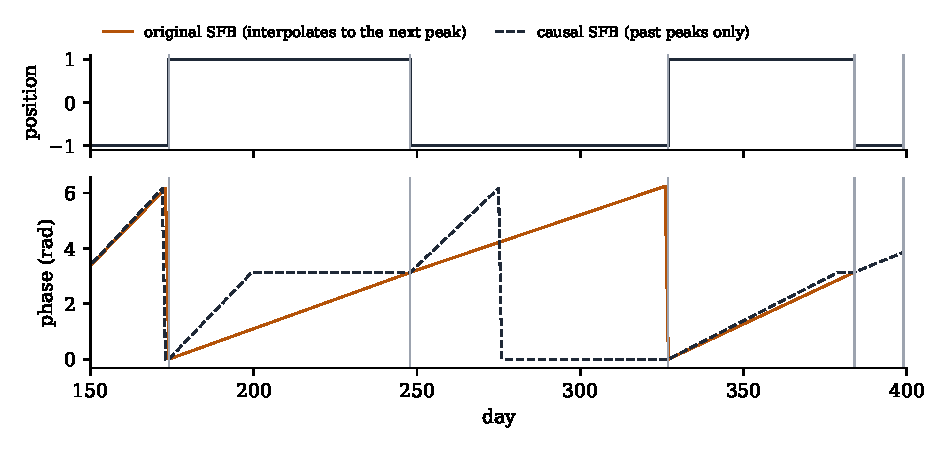
\includegraphics[width=\textwidth]{fig_lookahead.pdf}
\caption{Event-anchored phase on a position with irregular holding periods.
The interpolating phase (solid) reaches $\pi$ and $2\pi$ exactly at the next
reversal, which it cannot know at the time; the causal phase (dashed) uses past
bursts only and must guess the duration.}
\label{fig:lookahead}
\end{figure}

\subsection{A spread elasticity that is volatility on volatility}

Crowding models often rest on a liquidity elasticity $\beta$, estimated from
$\log V_t = \alpha - \beta\log\sigma_t + \varepsilon_t$ with $V_t$ the inverse
of a spread. When the spread is the \citet{Corwin2012} estimator, $V_t$ is a
function of the daily high-low range, itself a volatility estimator, and
$\beta$ is mechanically positive. We simulate a market whose true spread is
constant, so that liquidity never responds to volatility and the true $\beta$
is zero, and apply the estimator with a 21-day close-to-close $\sigma_t$. The
estimate is $\hat\beta = 0.87$ ($R^2 = 0.25$) with a zero spread, $0.81$ with
2~bp and $0.71$ with 10~bp: values typical of those reported on real futures
(a mean of 0.73 across 43 CME contracts in our earlier work). Quote-based
elasticities are not immune either: in our tick data, replacing contemporaneous
realized volatility by its one-day lag, to remove bid-ask bounce, leaves a rank
correlation of only 0.24 with the baseline estimates (24 of 43 signs change);
a 5-day median leaves 0.05.

\subsection{i.i.d.\ inference on overlapping horizons}
\label{sec:iid}

A 21-day forward drawdown sampled daily overlaps with its 20 neighbours, and
$r(t)$ is itself persistent (weekly AR(1) of 0.77 on real positions). A
standard rank-correlation $p$-value treats these observations as independent.
Table~\ref{tab:mc} shows what that does when nothing is predictable: 59--64\%
of the replications are ``significant'' at 5\%, and 18--23\% reach
$p < 10^{-6}$. The null correlations have a standard deviation of 0.07 and
reach $\pm 0.19$: in this design a correlation near 0.2 is roughly a
three-standard-deviation event, not a one-in-a-million one, and our earlier
headline figure ($\rho = 0.196$, reported with $p < 10^{-6}$, from a larger
but similarly overlapping design) sits at the edge of what pure noise produces
here. Every inference below uses a stationary block bootstrap \citep{Politis1994}
and Newey--West standard errors.

\section{A pre-registered test on real positions}
\label{sec:prereg}

\subsection{Data and design}

Positions are the weekly CFTC Commitments of Traders, futures only, Tuesday
as-of: leveraged funds in the Traders in Financial Futures report for equity
indices, Treasuries and currencies, managed money in the disaggregated report
for energy, metals, grains and livestock. The net position of market $i$ is
$x_i(t) = (\text{long} - \text{short})/\text{open interest}$. A report is used
from the first trading day on or after the Monday following its Tuesday as-of
date (it is released on Friday afternoon), and report weeks around the 2013,
2018--19 and 2025 government shutdowns, when releases were late, are excluded.
The universe is every market with at least 85\% coverage of both the CFTC
series (2009--2026) and our daily continuous futures (2010--2026): 32 markets.

The primary phase is causal and needs no event detection. With $z_i(t)$ the
156-week trailing z-score of $x_i$ and $d_i(t)$ the trailing z-score of its
weekly change,
\begin{equation}
\theta_i(t) = \operatorname{atan2}\bigl(-d_i(t),\, z_i(t)\bigr),
\end{equation}
so that $0$ is a maximal long, $\pi/2$ selling out of it, $\pi$ a maximal
short and $3\pi/2$ buying. Two secondary variants are reported without
decision weight: the nematic order parameter $|N^{-1}\sum_i e^{2i\theta_i}|$,
which treats long and short extremes as aligned, and the causal version of the
event-anchored phase of Section~\ref{sec:pitfalls}.

\textbf{H1} (synchronization exists): the mean of $r(t)$ exceeds the
distribution obtained by circularly shifting each market's phase series by an
independent random offset (2{,}000 surrogates), which keeps each market's own
dynamics and destroys cross-market alignment; threshold $p < 0.01$.

\textbf{H2} (synchronization precedes unwinds): in weekly regressions with
4-week horizons (770 weeks, entries 2010-08 to 2026-01), $r(t)$ predicts at
least one of: Y1, the return of the speculative book (each market long or
short with the sign of $x_i$, volatility-scaled, equal weight); Y2, its maximum
drawdown; Y3, the cross-market log ratio of forward to trailing realized
volatility. Controls: the book's trailing 4-week return, the trailing
volatility ratio, the mean pairwise correlation of position changes over 13
weeks, the first-principal-component share of position changes over 26 weeks,
and the mean absolute position z-score. Inference: stationary block bootstrap
(mean block 26 weeks, 5{,}000 draws) with a Romano--Wolf step-down across the
three outcomes \citep{RomanoWolf2005}; predicted signs $b<0$ for Y1 and Y2,
$b>0$ for Y3.

\textbf{H3} (out of sample): fit on entries to 2017, forecast 2018--2026, and
test against the model without $r(t)$ \citep{ClarkWest2007}.

The decision rule, fixed in advance: if H1 fails, the crowding claim is
abandoned; if H1 holds and H2 fails, synchronization is descriptive only; a
full crowding paper requires H1, H2 and H3.

\subsection{Results}

\begin{figure}[t]
\centering
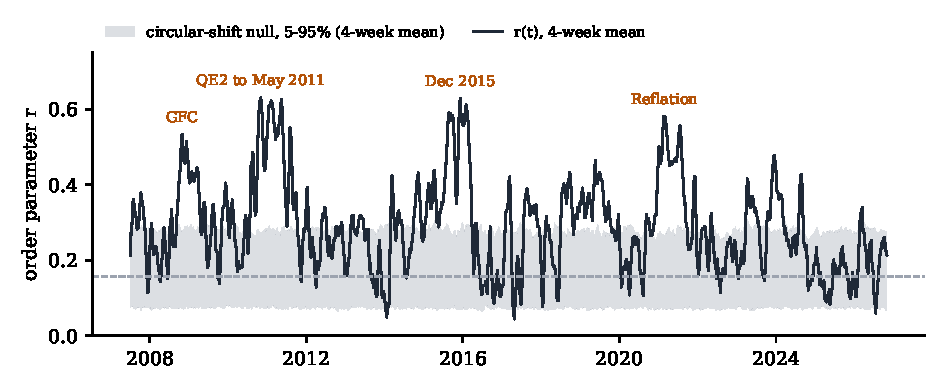
\includegraphics[width=\textwidth]{fig_r_real.pdf}
\caption{Order parameter of speculative positioning across 32 futures markets
(causal phase, 4-week mean) against the 5--95\% band of 500 circular-shift
surrogates.}
\label{fig:r}
\end{figure}

\paragraph{H1 holds.} The mean order parameter is 0.287 against a surrogate
mean of 0.156 (99th percentile 0.181; ratio 1.84; $p = 0.0005$, the smallest
attainable with 2{,}000 surrogates). The surrogate mean equals the i.i.d.\
floor $\sqrt{\pi/4N} = 0.157$, so the shifted series behave as independent
phases. Synchronization holds within financial markets (0.312 against 0.228)
and within commodities (0.368 against 0.225), and with the causal
event-anchored phase (0.211 against 0.156). Figure~\ref{fig:r} shows that it is
episodic: $r$ leaves the null band in late 2008, from the QE2 reflation trade
into the commodity sell-off of May 2011, at the end of 2015 and in early 2021.
The order parameter is nearly orthogonal to standard crowding proxies: its
Spearman correlation with the pairwise correlation of position changes is
$-0.05$, with the first-component share $-0.05$, with the mean absolute
position z-score $0.10$. It measures alignment in the position-and-flow plane,
which correlation of flows alone does not see.

\begin{table}[t]
\centering
\caption{Pre-registered predictive tests (H2, H3). Standardized coefficient
$b$ on $r(t)$ with controls; $t$ from Newey--West (8 lags); $p_{RW}$
Romano--Wolf adjusted from 5{,}000 stationary-bootstrap draws; Clark--West
one-sided $p$ and out-of-sample $R^2$ relative to the model without $r(t)$
(training to 2017, 396 test weeks).}
\label{tab:h2}
\small
\begin{tabular}{llrrrrr}
\toprule
Phase & Outcome & $b$ & $t_{NW}$ & $p_{RW}$ & $p_{CW}$ & $R^2_{oos}$ \\
\midrule
Primary & Y1 return      & $0.054$ & $0.71$ & $0.78$ & $0.40$ & $0.000$ \\
        & Y2 drawdown    & $-0.080$ & $-1.58$ & $0.33$ & $0.21$ & $0.005$ \\
        & Y3 vol. spike  & $-0.002$ & $-0.27$ & $0.78$ & $0.82$ & $-0.006$ \\
\addlinespace
Nematic & Y1 return      & $-0.128$ & $-1.91$ & $0.06$ & $0.08$ & $0.007$ \\
        & Y2 drawdown    & $-0.100$ & $-2.22$ & $0.02$ & $0.13$ & $0.006$ \\
        & Y3 vol. spike  & $0.000$ & $-0.01$ & $0.99$ & $0.56$ & $0.000$ \\
\addlinespace
Causal events & Y1 return & $-0.078$ & $-1.28$ & $0.39$ & $0.07$ & $0.002$ \\
        & Y2 drawdown    & $0.002$ & $0.05$ & $0.96$ & $0.51$ & $0.000$ \\
        & Y3 vol. spike  & $0.003$ & $0.35$ & $0.92$ & $0.80$ & $-0.008$ \\
\bottomrule
\end{tabular}
\end{table}

\paragraph{H2 and H3 fail.} Table~\ref{tab:h2} reports the predictive tests.
With the primary phase, no outcome comes close: adjusted $p$-values of 0.78,
0.33 and 0.78, and out-of-sample $R^2$ below one percent. The nematic variant,
which counts simultaneous long and short extremes as aligned, has the predicted
sign for drawdowns ($p_{RW} = 0.02$) but does not survive out of sample
($p_{CW} = 0.13$) and carries no weight under the pre-registered rule; we
report it as a lead for a separate, newly registered test.

\paragraph{A disclosed first run.} Our first run loaded only the 2006--2016
financial archive because of a file-name pattern, and its universe was the 16
commodity markets. On that sub-universe the primary order parameter predicts
4-week returns of the speculative book with the \emph{opposite} sign to the
crowding thesis ($b = 0.33$, $t_{NW} = 3.20$, $p_{RW} = 0.004$; out of sample
$p_{CW} = 0.02$): synchronized commodity positioning was followed by
continuation, not unwinding. The bug was fixed, documented in a dated
amendment, and the 32-market run is the registered result; we mention the
commodity result because it shows how much a single universe choice can
change the conclusion.

\section{Conclusion}

Real speculative positions phase-lock across futures markets, in identifiable
episodes, and the Kuramoto order parameter captures an alignment that
correlation-based crowding measures miss. None of this translates into a
warning: in a pre-registered design with point-in-time data, synchronization
predicts neither losses, nor drawdowns, nor volatility of the speculative book.
Studies that report the opposite should show that their phases are causal
(an alteration test costs one line), that their liquidity elasticities are not
built from volatility, and that their inference respects overlapping horizons.

\bibliographystyle{plainnat}
\begin{thebibliography}{9}
\bibitem[Acebr\'on et~al.(2005)]{Acebron2005}
Acebr\'on, J.~A., Bonilla, L.~L., P\'erez Vicente, C.~J., Ritort, F., and Spigler, R. (2005).
The Kuramoto model: A simple paradigm for synchronization phenomena.
\emph{Reviews of Modern Physics}, 77(1):137--185.
\bibitem[Brunnermeier and Pedersen(2009)]{Brunnermeier2009}
Brunnermeier, M.~K. and Pedersen, L.~H. (2009).
Market liquidity and funding liquidity.
\emph{Review of Financial Studies}, 22(6):2201--2238.
\bibitem[Clark and West(2007)]{ClarkWest2007}
Clark, T.~E. and West, K.~D. (2007).
Approximately normal tests for equal predictive accuracy in nested models.
\emph{Journal of Econometrics}, 138(1):291--311.
\bibitem[Corwin and Schultz(2012)]{Corwin2012}
Corwin, S.~A. and Schultz, P. (2012).
A simple way to estimate bid-ask spreads from daily high and low prices.
\emph{Journal of Finance}, 67(2):719--760.
\bibitem[Pedersen(2009)]{Pedersen2009}
Pedersen, L.~H. (2009).
When everyone runs for the exit.
\emph{International Journal of Central Banking}, 5(4):177--199.
\bibitem[Politis and Romano(1994)]{Politis1994}
Politis, D.~N. and Romano, J.~P. (1994).
The stationary bootstrap.
\emph{Journal of the American Statistical Association}, 89(428):1303--1313.
\bibitem[Romano and Wolf(2005)]{RomanoWolf2005}
Romano, J.~P. and Wolf, M. (2005).
Stepwise multiple testing as formalized data snooping.
\emph{Econometrica}, 73(4):1237--1282.
\bibitem[Strogatz(2000)]{Strogatz2000}
Strogatz, S.~H. (2000).
From Kuramoto to Crawford: exploring the onset of synchronization in populations of coupled oscillators.
\emph{Physica D}, 143(1--4):1--20.
\end{thebibliography}

\end{document}
